
\chapter{Systems of PDEs, and the Stokes equations}
\label{chap:stokes}

\section{First-order systems}

FIXME: FOSLS for Poisson?

\section{Stokes equations}

FIXME: lay out theory 

Thus the incompressible variable-viscosity Navier-Stokes has these main equations
\begin{align*}
\rho \left(\frac{\partial \bu}{\partial t} + \bu \cdot \grad \bu\right) &= \Div \sigma + \bg \\
\sigma &= 2 \nu\, Du - p I \\
\Div \bu &= 0
\end{align*}
where
  $$\grad \bu = \renewcommand{\arraystretch}{1.3}\begin{bmatrix}
    \frac{\partial u_1}{\partial x} & \frac{\partial u_2}{\partial x} & \frac{\partial u_3}{\partial x} \\
    \frac{\partial u_1}{\partial y} & \frac{\partial u_2}{\partial y} & \frac{\partial u_3}{\partial y} \\
    \frac{\partial u_1}{\partial z} & \frac{\partial u_2}{\partial z} & \frac{\partial u_3}{\partial z}
    \end{bmatrix}$$
and
    $$D u = \frac{1}{2} \left(\grad \bu + \grad \bu^{\top}\right).$$

FIXME: theory where Froude $\approx 0$

Thus the variable-viscosity Stokes equations, in terms of velocity, are
\begin{align*}
\Div \left(\nu \left(\grad \bu + \grad \bu^{\top}\right)\right) - \grad p &= - \bg \\
\Div \bu &= 0
\end{align*}

We will, however, first consider the case where the viscosity $\nu$ is constant.  In such case the velocity second derivative term can be simplified, and recognized as an application of the Laplacian operator.  Observe that by commuting mixed derivatives and using incompressibility we have
\begin{align*}
\Div \left(\grad \bu^{\top}\right) &= \renewcommand{\arraystretch}{1.3}\begin{bmatrix}
    \frac{\partial}{\partial x} & \frac{\partial}{\partial y} & \frac{\partial}{\partial z}
    \end{bmatrix}
    \begin{bmatrix}
    \frac{\partial u_1}{\partial x} & \frac{\partial u_1}{\partial y} & \frac{\partial u_1}{\partial z} \\
    \frac{\partial u_2}{\partial x} & \frac{\partial u_2}{\partial y} & \frac{\partial u_2}{\partial z} \\
    \frac{\partial u_3}{\partial x} & \frac{\partial u_3}{\partial y} & \frac{\partial u_3}{\partial z}
    \end{bmatrix} \\
  &= \begin{bmatrix}
    \frac{\partial}{\partial x}\left(\Div \bu\right) & \frac{\partial}{\partial y }\left(\Div \bu\right) & \frac{\partial}{\partial x} \left(\Div \bu\right)
    \end{bmatrix}
    = 0.
\end{align*}
On the other hand,
\begin{align*}
\Div \left(\grad \bu\right) &= \renewcommand{\arraystretch}{1.3}\begin{bmatrix}
    \frac{\partial}{\partial x} & \frac{\partial}{\partial y} & \frac{\partial}{\partial z}
    \end{bmatrix}
    \begin{bmatrix}
    \frac{\partial u_1}{\partial x} & \frac{\partial u_2}{\partial x} & \frac{\partial u_3}{\partial x} \\
    \frac{\partial u_1}{\partial y} & \frac{\partial u_2}{\partial y} & \frac{\partial u_3}{\partial y} \\
    \frac{\partial u_1}{\partial z} & \frac{\partial u_2}{\partial z} & \frac{\partial u_3}{\partial z}
    \end{bmatrix} \\
  &= \begin{bmatrix} \grad^2 u_1 & \grad^2 u_2 & \grad^2 u_3 \end{bmatrix} = \grad^2 \bu
\end{align*}
which we have written as ``$\grad^2 \bu$,'' that is, the last equality is a definition.  

Thus we have a Poisson-like problem for $\bu$, but with an unknown pressure playing a role as a source term, in addition to the body force $\bg$.  For consistency with the Poisson equation sign convention in Chapters \ref{chap:structured}--\ref{chap:multigrid}, in the constant viscosity case we write the Stokes equations as
\begin{align}
- \nu \grad^2 \bu + \grad p &= \bg \\
\Div \bu &= 0
\end{align}


\section{Fluid flowing down a slope}

FIXME: reduce to 2D with gravity body force.

The particular problem we will solve is a constant-thickness flow down a slope of angle $\theta$, using rotated coordinates as in Figure \ref{fig:slabonslope}.  First we simplify the appearance of the field equations.  Write $u=u_1$ and $v=u_2$.  Then the three scalar equations are
\begin{align}
-\nu \grad^2 u + p_x &= g_1 \label{stokes2du} \\
-\nu \grad^2 v + p_y &= g_2 \label{stokes2dv} \\
u_x + u_y &= 0 \label{stokes2dincomp}
\end{align}
where $\nu$ is constant and $\bg = (g_1,g_2) = (\rho g \sin \theta, - \rho g \cos \theta)$.

\begin{marginfigure}
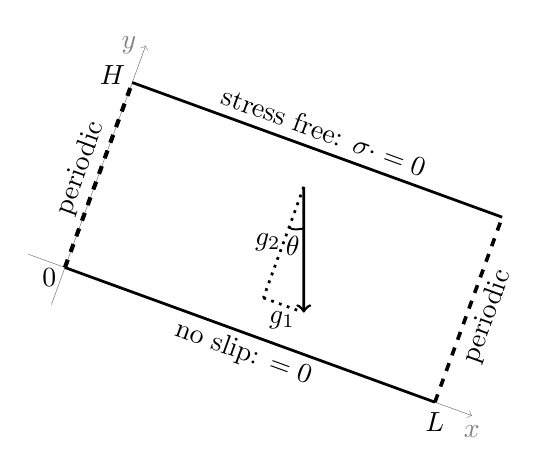
\begin{tikzpicture}[scale=2.5,rotate=-20]
  \draw[->,gray,very thin] (-0.2,0.0) -- (2.2,0.0) node[below] {$x$};
  \draw[->,gray,very thin] (0.0,-0.2) -- (0.0,1.2) node[left] {$y$};
  \node[xshift=-0.2cm,yshift=-0.13cm] at (0.0,0.0) {$0$};
  \node[xshift=0.0cm,yshift=-0.25cm] at (2.0,0.0) {$L$};
  \node[xshift=-0.25cm,yshift=0.1cm] at (0.0,1.0) {$H$};
  \draw[line width=1.0pt] (0.0,0.0) -- (2.0,0.0);
  \draw[line width=1.0pt] (0.0,1.0) -- (2.0,1.0);
  \node[rotate=-20] at (1.0,-0.1) {no slip: $\bu=0$};
  \node[rotate=-20] at (1.0,1.1) {stress free: $\sigma\cdot\bn=0$};
  \draw[line width=1.5pt,dashed] (0.0,0.0) -- (0.0,1.0);
  \draw[line width=1.3pt,dashed] (2.0,0.0) -- (2.0,1.0);
  \node[rotate=70] at (-0.1,0.5) {periodic};
  \node[rotate=70] at (2.1,0.5) {periodic};
  \draw[line width=1.0pt,dotted] (1.0,0.8) -- node[xshift=-0.2cm,yshift=0.0cm] {$g_2$} (1.0,0.2);
  \draw[line width=1.0pt,dotted] (1.0,0.2) -- node[xshift=0.0cm,yshift=-0.2cm] {$g_1$} (1.2,0.2);
  %>> 0.6 * tan((pi/180)*20)
  %ans =  0.21838
  \draw[->,line width=1.0pt] (1.0,0.8) -- (1.21838,0.2) node[xshift=0.2cm,yshift=0.6cm] {$\bg$};
  \draw[line width=0.7pt] (1.0,0.58) .. controls (1.03,0.575) and (1.04,0.585) .. (1.07,0.6);
  \node at (1.05,0.5) {$\theta$};
\end{tikzpicture}
\caption{Geometry and boundary conditions of our first Stokes problem, for sticky fluid flowing down a slope.}
\label{fig:slabonslope}
\end{marginfigure}

Because the flow is actually intended to be infinite in the $x$ direction, for a numerical approximation we will require the solution to be periodic in $x$, so the domain is the rectangle $[0,L]\times[0,H]$ (in the rotated coordinates), where $H$ is the thickness and $L$ the length.  We assume a stress-free top and no slip at the base.  Because the normal direction to the top is in the (rotated) $y$-direction, the top boundary condition is
  $$\sigma\cdot\bn = 0 \iff
\begin{bmatrix}
2 \nu u_x - p & \nu (u_y+v_x) \\
\nu (u_y+v_x) & 2 \nu v_y - p
\end{bmatrix} \begin{bmatrix}
0 \\ 1
\end{bmatrix} = \begin{bmatrix}
0 \\ 0
\end{bmatrix}.$$
Thus, with the no-slip base, we have these boundary conditions,
\begin{align}
\text{top $y=H$:}&    & &\begin{array}{l} u_y + v_x = 0 \\ 2 \nu v_y = p\end{array}  \label{bcstokestop} \\
\text{bottom $y=0$:}& & &\begin{array}{l} u = 0 \\ v = 0 \end{array} \label{bcstokesbottom} \\
\text{sides $x=0$ and $x=L$:}&
                      & &u,v,p \text{ are periodic}. \label{bcstokesperiodic}
\end{align}


\section{Block structure of numerical Stokes solvers}

FIXME: Laplacians are something we understand, so lets proceed with eqns \eqref{stokes2du}, \eqref{stokes2dv}

FIXME: any way we do \eqref{stokes2dincomp} we get block structure for the full system ``$A \bz = \bbf$.''  Informally the structure is
  $$\begin{bmatrix}
    -\nu\grad^2 & 0 & \partial/\partial x \\
    0 & -\nu\grad^2 & \partial/\partial y \\
    \partial/\partial x & \partial/\partial y & 0
    \end{bmatrix}
    \begin{bmatrix}
    \bu \\ \bv \\ \bp
    \end{bmatrix}
    =
    \begin{bmatrix}
    g_1 \\ g_2 \\ 0
    \end{bmatrix}
    $$
but let's write
  $$\begin{bmatrix}
    \nu L_1 & 0 & G_1 \\
    0 & \nu L_2 & G_2 \\
    B_1 & B_2 & 0
    \end{bmatrix}
    \begin{bmatrix}
    \bu \\ \bv \\ \bp
    \end{bmatrix}
    =
    \begin{bmatrix}
    g_1 \\ g_2 \\ 0
    \end{bmatrix}
    $$
where $L_i$, $G_i$, $B_i$ are matrices.  We expect that Laplacian-approximation matrices $L_1$ and $L_2$, which essentially differ only in their boundary conditions, can be built as symmetric positive-definite matrices.

FIXME: $A$ certainly not invertible if approx to ``$\Div \bu$'' (i.e.~$\begin{bmatrix} B_1 & B_2 \end{bmatrix}$) has more rows than columns

FIXME: extract approx to ``$\Div \bu$'' as transpose of the ``$\grad p$'' part (i.e.~$\begin{bmatrix} G_1 \\ G_2 \end{bmatrix}$)
    $$\begin{bmatrix}
    \nu L_1 & 0 & G_1 \\
    0 & \nu L_1 & G_2 \\
    G_1^\top & G_2^\top & 0
    \end{bmatrix}
    \begin{bmatrix}
    \bu \\ \bv \\ \bp
    \end{bmatrix}
    =
    \begin{bmatrix}
    g_1 \\ g_2 \\ 0
    \end{bmatrix}$$
Now system is symmetric, but not positive definite.

Before proceeding let us observe that the pressure can be seen to solve its own equation, at least assuming smoothness of the solution to \eqref{stokes2du}--\eqref{stokes2dincomp}.  By taking the $x$ and $y$ derivatives of \eqref{stokes2dincomp} we get equations
\begin{align*}
u_{xx} + v_{yx} &= 0, \\
u_{xy} + v_{yy} &= 0.
\end{align*}
These allow us to replace $u_{xx}$ and $v_{yy}$ in \eqref{stokes2du}, \eqref{stokes2dv} with mixed derivatives, respectively, to get:
\begin{align}
-\nu \left(-v_{yx} + u_{yy}\right) + p_x &= g_1 \label{mixedstokes2du} \\
-\nu \left(v_{xx} - u_{xy}\right) + p_y &= g_2 \label{mixedstokes2dv}
\end{align}
Now, taking the $x$ derivative of \eqref{mixedstokes2du} and the $y$-derivative of \eqref{mixedstokes2dv}, and noting $g_i$ are constant, and adding the results, the velocity derivatives cancel entirely.  We conclude that $p$ actually solves Laplace's equation,
\begin{equation}
\grad^2 p = 0. \label{pressurepoisson}
\end{equation}
The derivation here is not original; we have arrived at the \emph{pressure-Poisson} equation \citep{Ockendonetal2003}.

The appearance of the Laplacian in a decoupled equation opens up the possibility that we can make our linear system ``more positive definite'' by adding a multiple of equation \eqref{pressurepoisson} to the Stokes system.  Concretely, if $\eps\ge 0$ then this system is equivalent to \eqref{stokes2du}--\eqref{stokes2dincomp}:
\begin{align}
-\nu \grad^2 u + p_x &= g_1 \label{ppstokes2du} \\
-\nu \grad^2 v + p_y &= g_2 \label{ppstokes2dv} \\
u_x + u_y - \eps \grad^2 p &= 0 \label{ppstokes2dincomp}
\end{align}
These equations correspond to block structure of the numerical approximation,
\begin{equation}
\begin{bmatrix}
    \nu L_1 & 0 & G_1 \\
    0 & \nu L_1 & G_2 \\
    G_1^\top & G_2^\top & \eps L_3
    \end{bmatrix}
    \begin{bmatrix}
    \bu \\ \bv \\ \bp
    \end{bmatrix}
    =
    \begin{bmatrix}
    g_1 \\ g_2 \\ 0
    \end{bmatrix} \label{blockppstokes}
\end{equation}
which we write as $A\bz = \bbf$ for the rest of this Chapter.  We show parameters $\nu>0$ and $\eps \in \RR$ to emphasize that we can play with problems of different viscosity and with more or less pressure-Poisson regularization, respectively. 


\section{A finite difference, structured-grid approach}

In this section we apply centered finite differences to equations \eqref{ppstokes2du}--\eqref{ppstokes2dincomp} using boundary conditions \eqref{bcstokestop}--\eqref{bcstokesperiodic} to get a symmetric linear system with block structure \eqref{blockppstokes}.

FIXME: not the best way but illuminating; code uses DMDA and SNES


\section{Preconditioners for indefinite systems}

FIXME: while $A$ is symmetric, it is not positive definite; note that if
    $$M = \begin{bmatrix} 0 & G \\ G^\top & 0 \end{bmatrix}$$
and if $M$ has eigenvalue $\lambda$ so that
    $$M \begin{bmatrix} \bx \\ \by \end{bmatrix} = \lambda \begin{bmatrix} \bx \\ \by \end{bmatrix}$$
then
    $$M \begin{bmatrix} -\bx \\ \by \end{bmatrix} = - \lambda \begin{bmatrix} -\bx \\ \by \end{bmatrix}$$
and (w.o.l.o.g.) this is a lin.-indep. eigenvector so $M$ also has eigenvalue $-\lambda$



\caveat{But \PETSc should help with unstructured meshes too.}

